\section{Selection}

Signal candidates for the decays \btokpipimumu and \btophikmumu must first pass the \lone trigeer
line {\tt L0Muon}.
Subsequent software trigger stages required that at least one final-state muon has $\pt>1.6\gev$
and at least one hadron has $\pt>1.0\gev$, both of which had an IP larger than $100\mum$ with
respect to any PV in the event.
The responce of the topological BBDT in the \hlttwo must be consistent with a decaying $B$ meson
with muons in the final state.

%There is large overlap between the...

Candidate \Bp hadrons are then formed from combinations of three hadrons and a pair of opposite
sign nuons.
Fully reconstructed candidates must form a good quiality vertex, with a \chisq of the vertex fit
$<6$.
This secondary vertex must be well displaced from any PV, having a flight distance inconsistent
with zero; ($\chisqfd>121$).
The angle between the \Bp candidate momentum vector and the directon defined by the PV to \Bp decay
vertex must be less than $14\mrad$.
Each track must satisfy $\chisqip>16$, where the \chisqip of a track is defined as the change in
\chisqip when calculated with and withoug the track in question.
The muons must both satisfy the {\tt isMuon} criteria and have $\dllmupi>0$.
Hadrons have PID criteria applied later, after optimization, but the total invariant mass of the
\kpipi system is required to be below $2400\mev$.
Each hadron must have $\pt>500\gev$.
For the \phik system, the additional constraint that the \decay{\phi}{\kk} object must have an
invariant mass within $12\mev$ of $m_\phi^\pdg$.



\subsection{Irriducible backgrounds}

Processes with the same final state as \btokpipimumu and \btophikmumu are not smoothly distributed
in $m_{K\pi\pi\mu\mu}$, rather they peak under the signal.


The tree level decays \decay{\Bp}{\jpsi\kpipi} and \decay{\Bp}{\jpsi\phik}, where
\decay{\jpsi}{\mumu}, have large branching fractions:
\begin{align}
  \BF(\decay{\Bp}{\jpsi(\to\mumu)\kpipi}) &= (4.8 \pm 0.8)\e{-5} \\
  \BF(\decay{\Bp}{\jpsi(\to\mumu)\phik}) &= (3.1 \pm 1.1)\e{-6},
\end{align}
and the same final state particles.
The same is true for the large contributions from \decay{\Bp}{\psitwos\kpipi} and
\decay{\Bp}{\psitwos\phik} decays, where \decay{\psitwos}{\mumu}.
These constitute large, irriducible backgrounds and must be removed with veotes around the \jpsi
and \psitwos masses.
However, the amount of contamination from decaying \jpsi and \psitwos is so great that both show
evidence of asymmetric tails from


\begin{figure}
  \begin{center}
    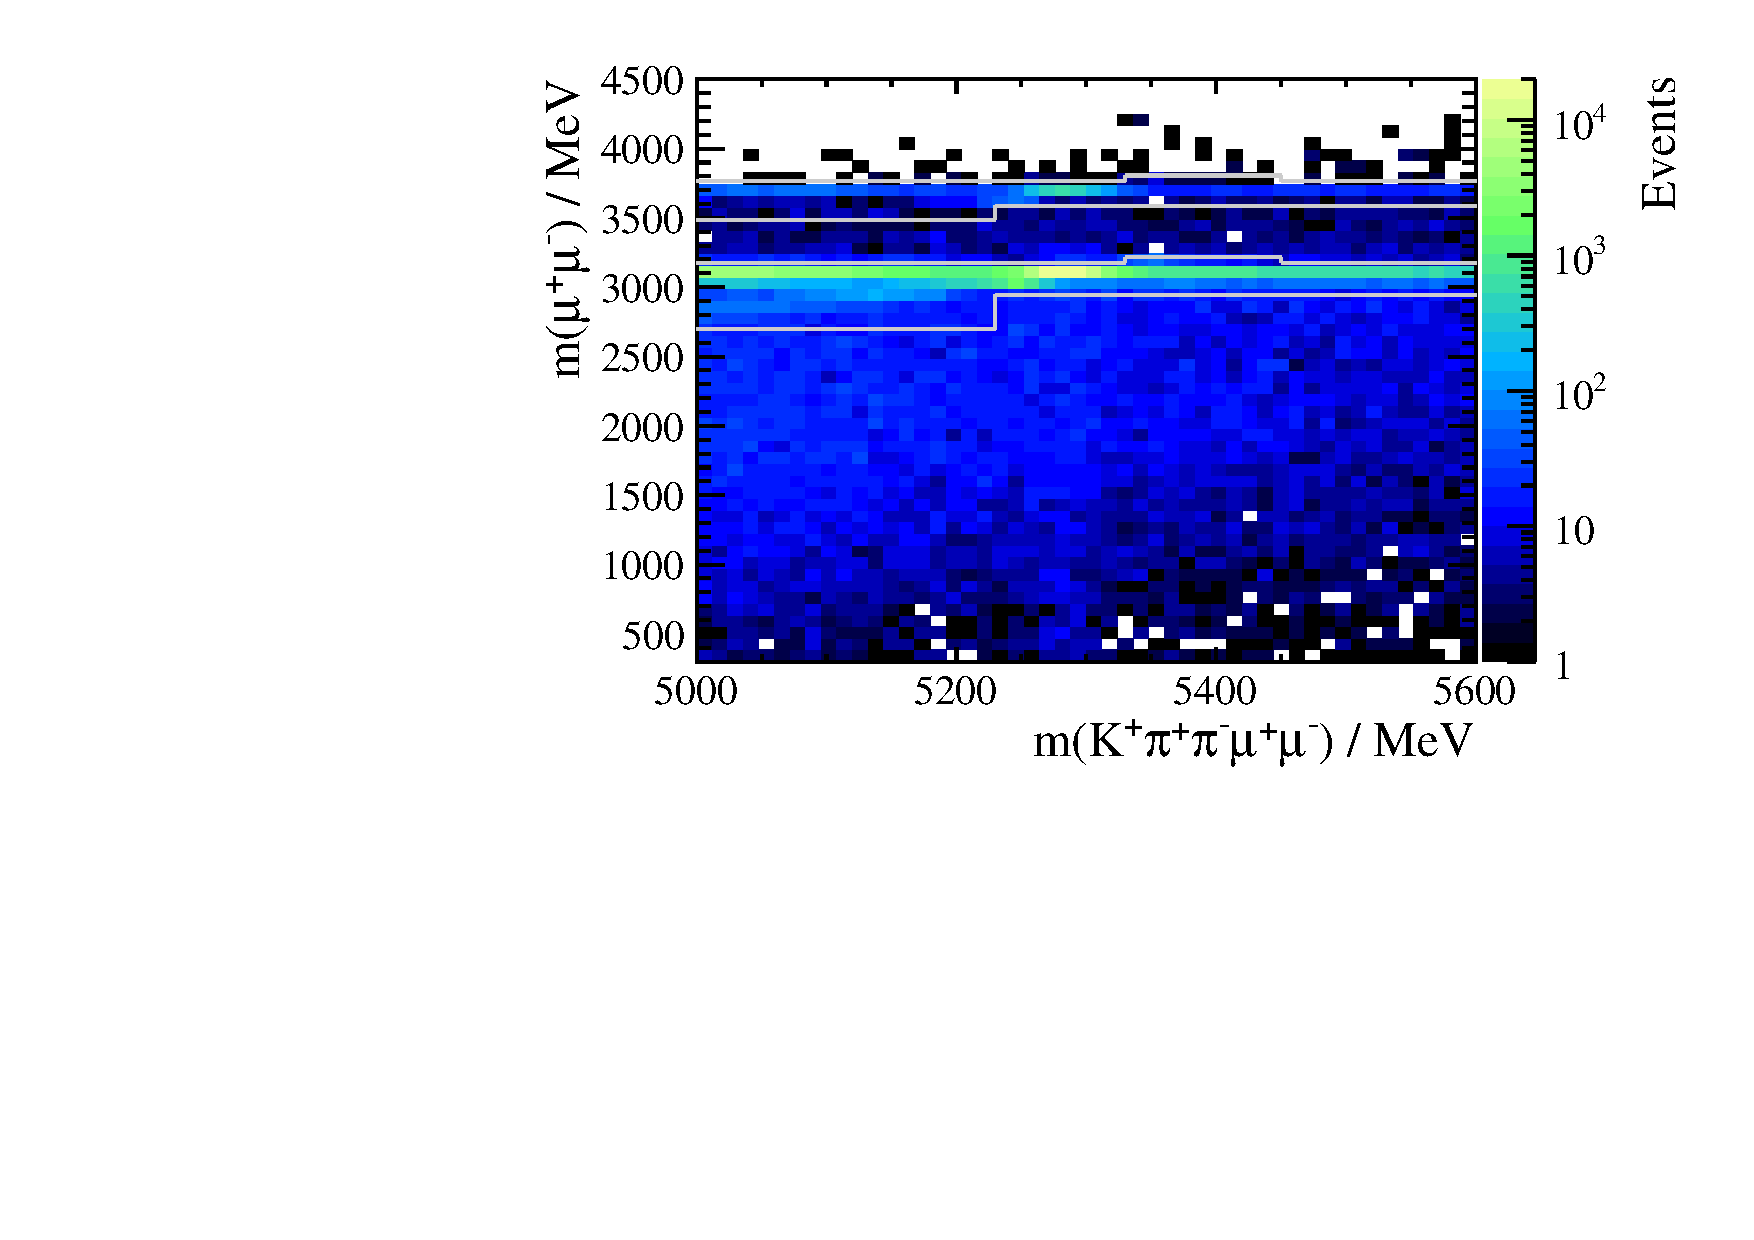
\includegraphics[width=0.45\textwidth]{BvJpre}
    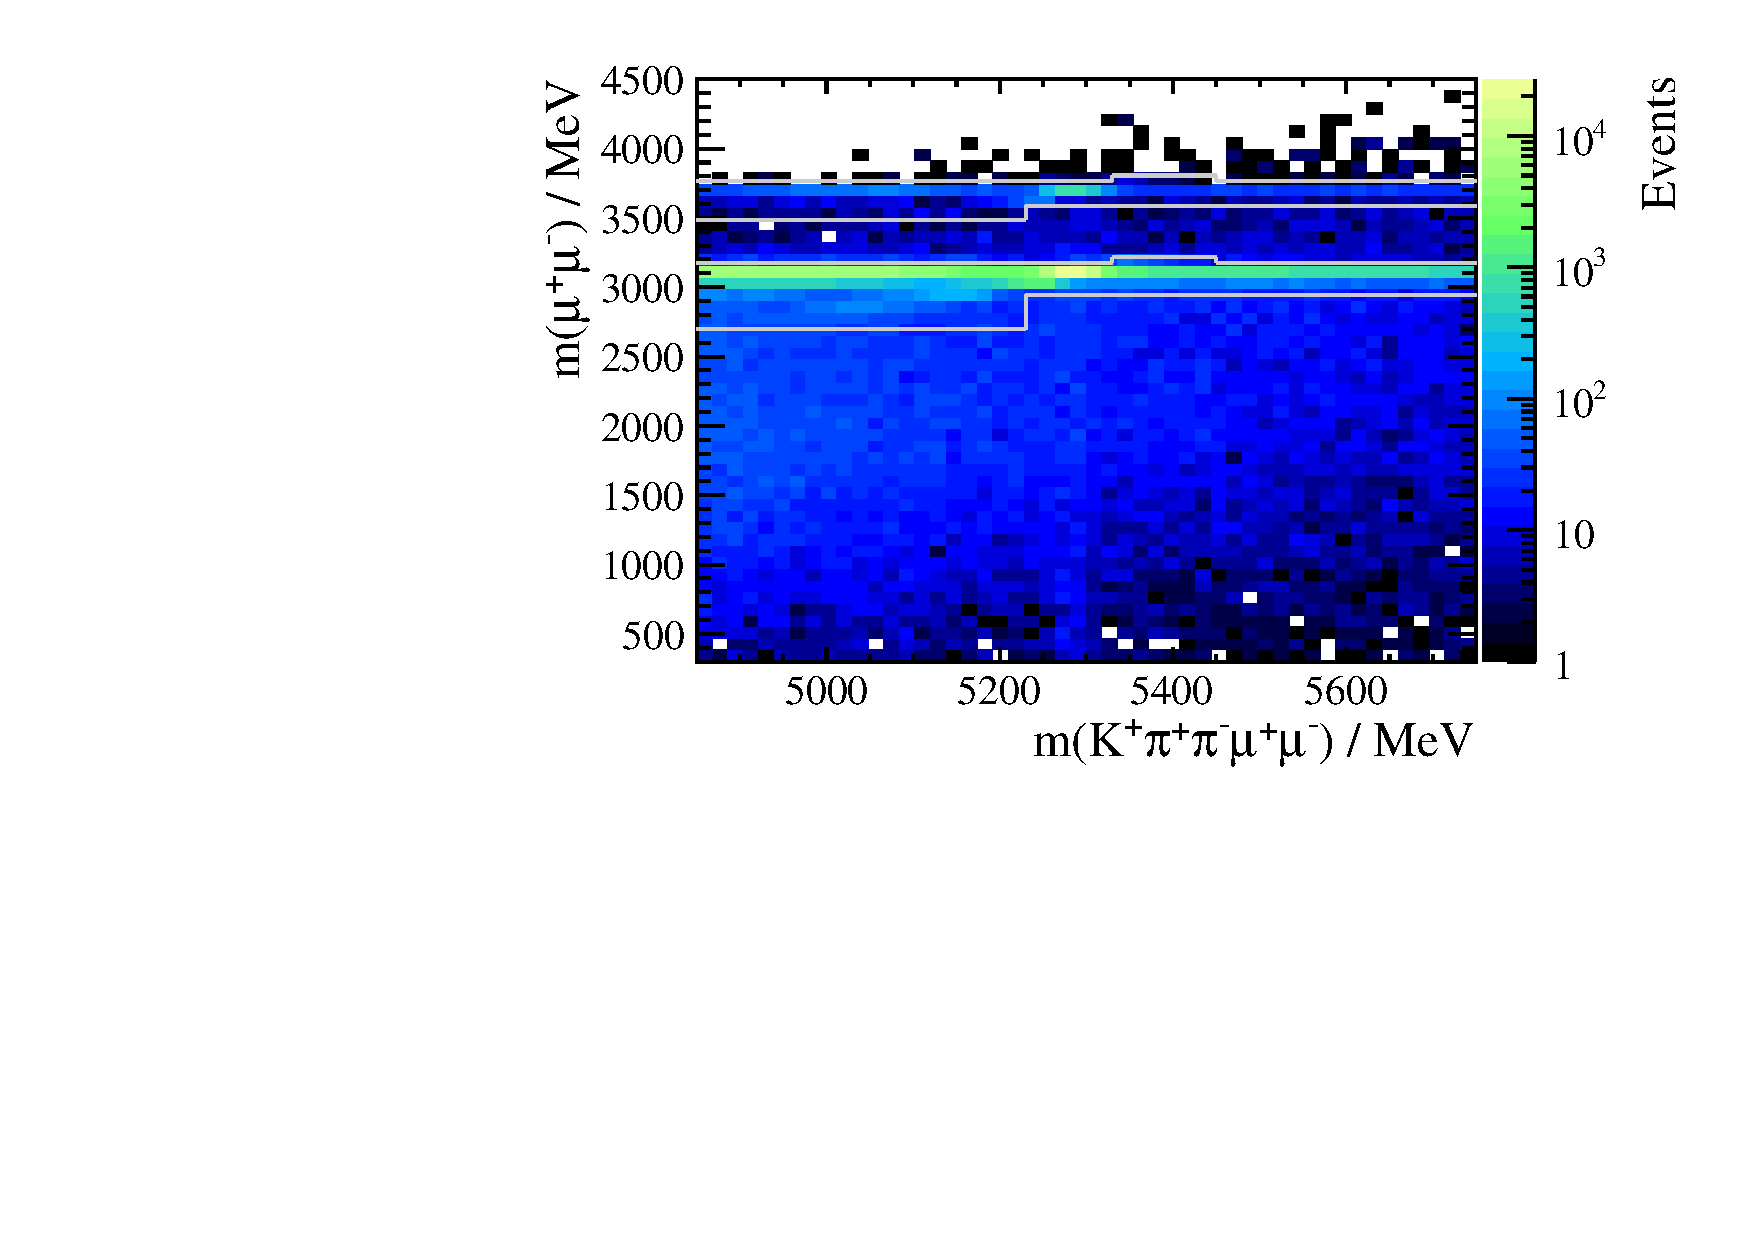
\includegraphics[width=0.45\textwidth]{BvJpost}\\
    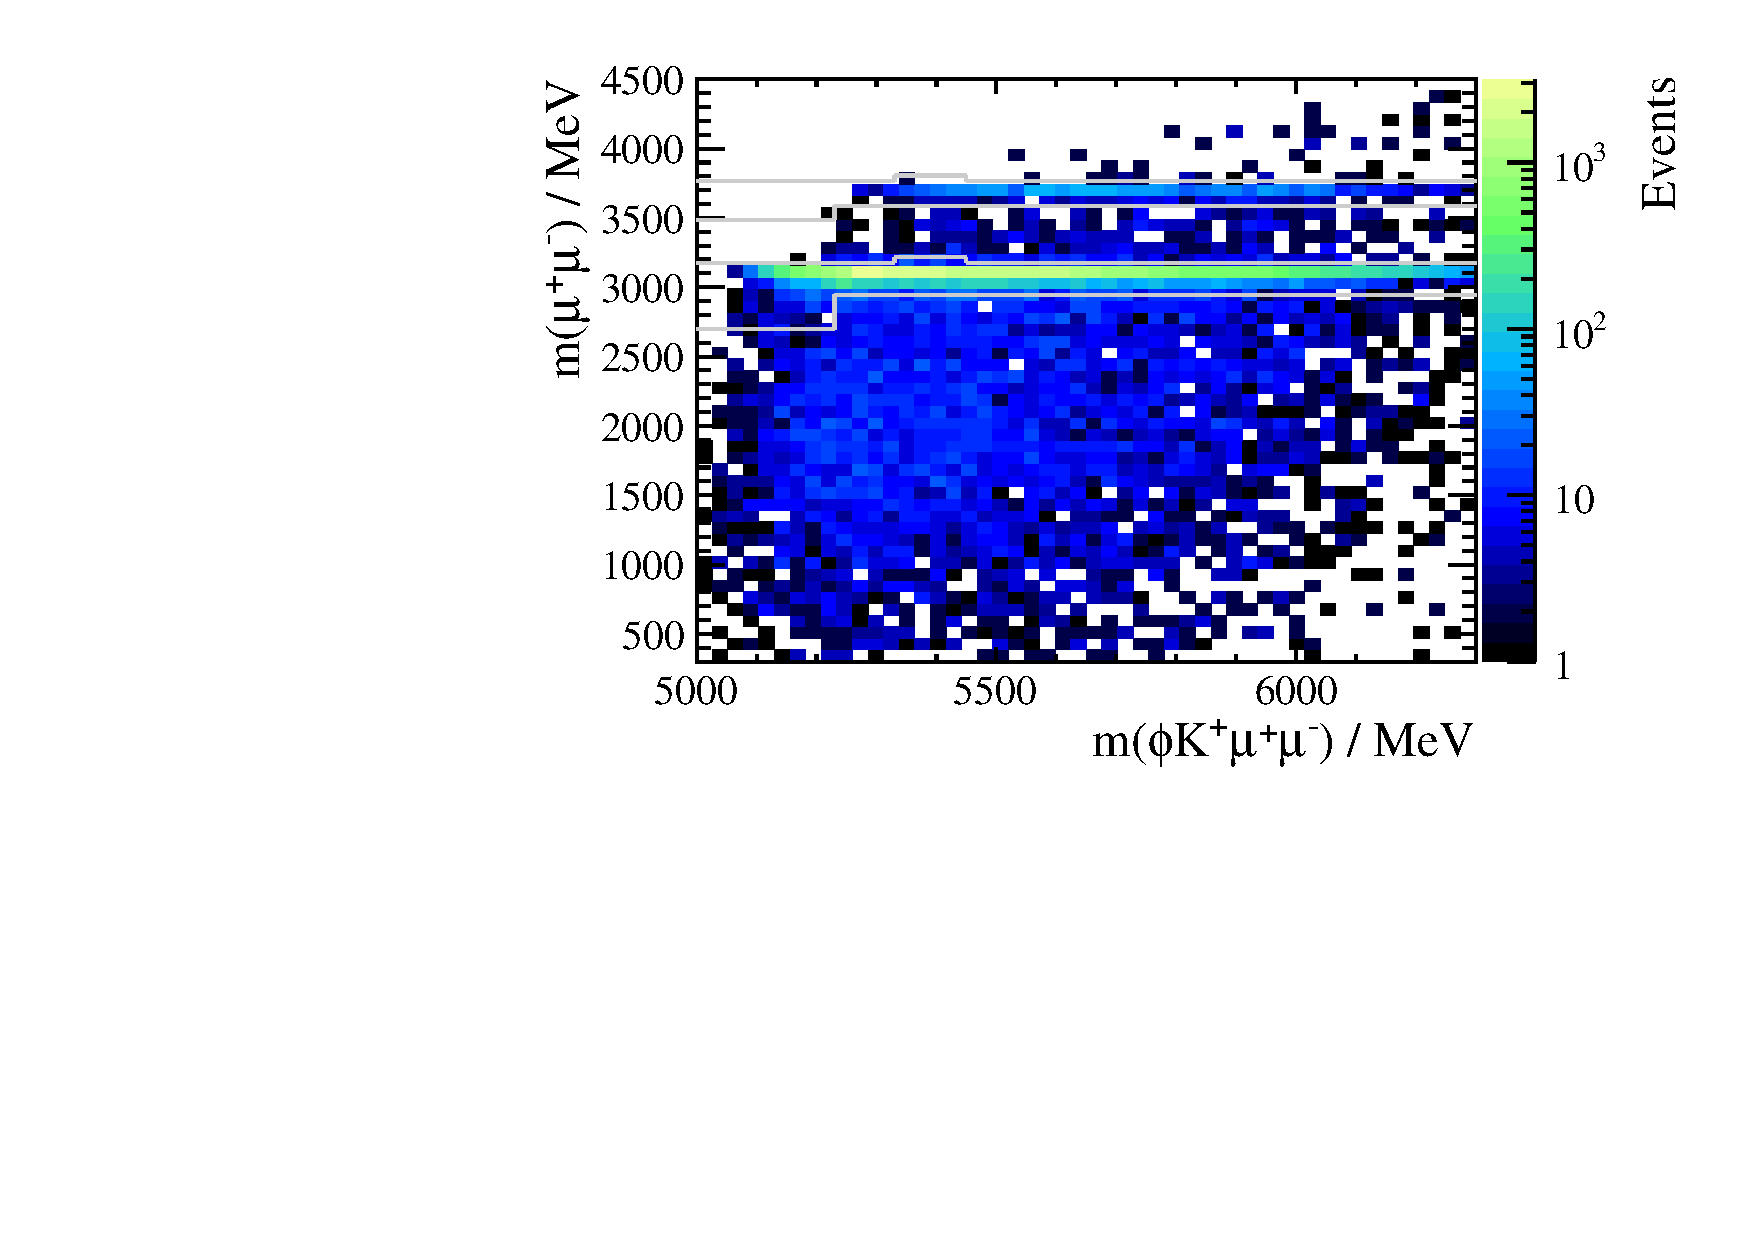
\includegraphics[width=0.45\textwidth]{BvJkkkpre}
    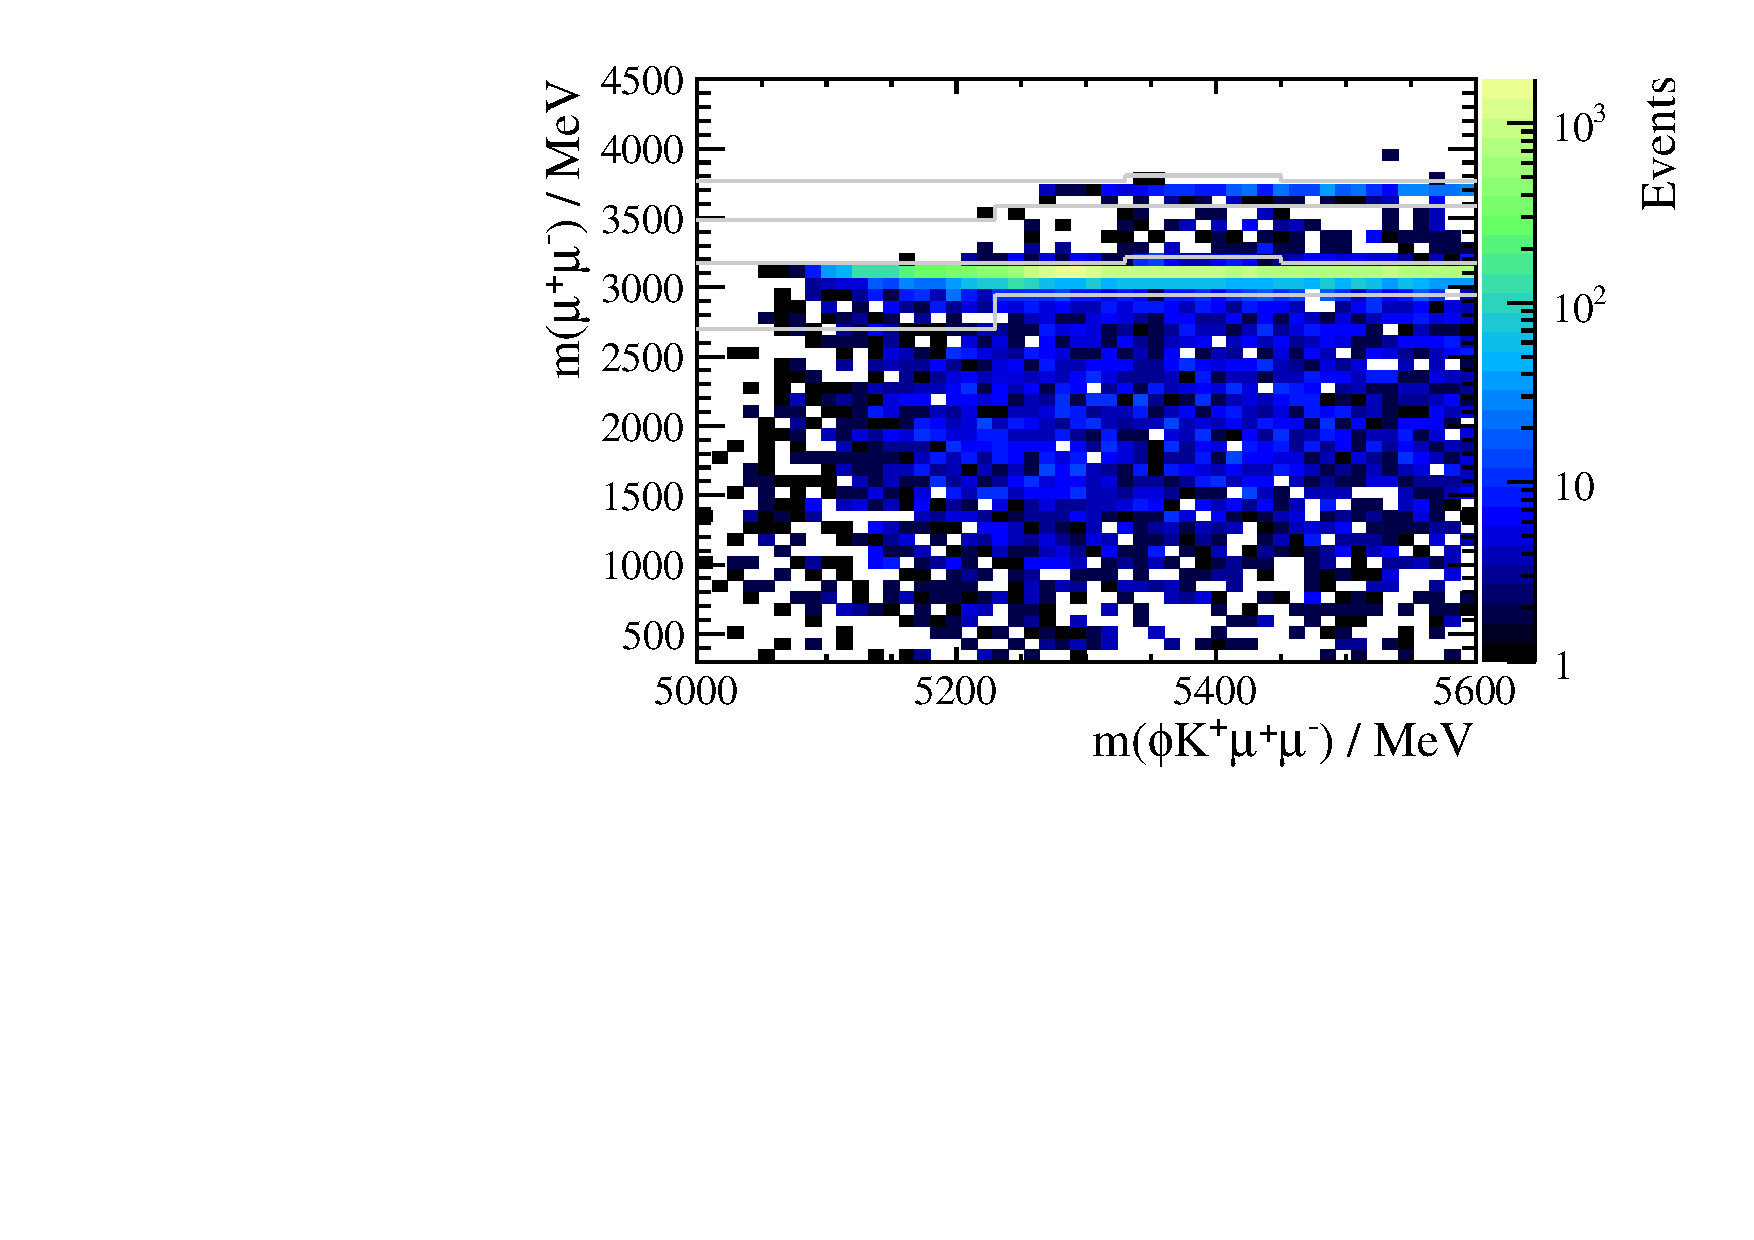
\includegraphics[width=0.45\textwidth]{BvJkkkpost}
    \caption{\small
      Charmonium vetoes.
    }
    \label{fig:hhh:charmvetoes}
  \end{center}
\end{figure}



%PID info from the RICH is used to identify final state hadrons
%PV chosen based on lowest PV of B candidateo
%vertex fit \chisq must increase by more than 121 when including the B candidate daughters
%fit vertex chi2 < 6

%Backgorunds of \jpsi and \psitwos must be removed
%also their radiative tails

%main sources of peaking backgrounds come from charmonia

\subsection{Multivariate selection}

%\section{Backgrounds}
%\section{Mass fits}
%\section{Efficiencies}
%\section{Systematics}
%\section{Summary}
